\documentclass{article}
\include{graphicx}


\begin{document}

\title{Review of OpenMP and MPI code}
\author{Joshua Wallace}

\maketitle

The plots I made for the analysis portion of this homework are 3-d ``wire'' plots.  I think they make sense once you see them.  I did not know how to put axes on them so I wish to explain here what the axes are on each of the plots.  The vertical axis is the temperature T for each plot, while the bottom left axis in the foreground is x and the bottom right axis in the foreground is y.

Figure~\ref{fig:1} shows the temperature as a function of position for the serial run with grid size of 128.  Looks pretty good.  Figure~\ref{fig:2} shows the same for the serial 256 grid size run and Figure~\ref{fig:3} is the same for the serial 512 grid size run.  The average temperatures for each run are as follows: 128, 0.496830306313; 256, 0.49695963511; 512, 0.497022899482.
\begin{figure}
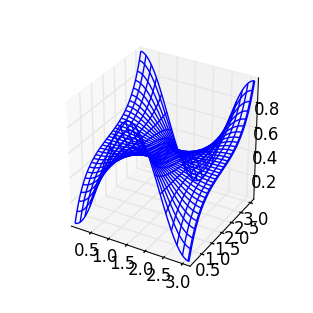
\includegraphics[width=85mm]{serial_128.png}
\caption{\label{fig:1}Temperature as a function of position for the serial run with grid size of 128. The vertical axis is the temperature T, while the bottom left axis in the foreground is x and the bottom right axis in the foreground is y.}
\end{figure}
\begin{figure}
%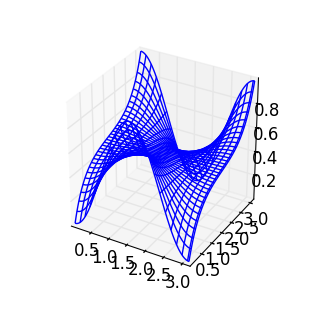
\includegraphics[width=85mm]{serial_256.png}
\caption{\label{fig:2}Temperature as a function of position for the serial run with grid size of 256. The vertical axis is the temperature T, while the bottom left axis in the foreground is x and the bottom right axis in the foreground is y.}
\end{figure}
\begin{figure}
%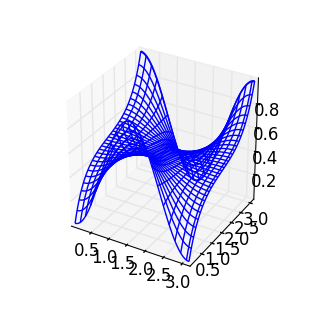
\includegraphics[width=85mm]{serial_512.png}
\caption{\label{fig:3}Temperature as a function of position for the serial run with grid size of 512. The vertical axis is the temperature T, while the bottom left axis in the foreground is x and the bottom right axis in the foreground is y.}
\end{figure}


The OpenMP runs had the same exact output data as the serial runs no matter how many numbers of threads I set for the OpenMP run.  Thus, I decided to not waste space or time by including the same looking figures again.  Please refer to Figures~\ref{fig:1}, \ref{fig:2}, and \ref{fig:3} for the corresponding plots for grid size of 128, 256, and 512, respectively, irrespective of number of threads.  Similarly the average temperatures for the various runs all correspond with the temperatures I gave for the serial cases.




\end{document}
